\begin{figure}[H]
	\centering
	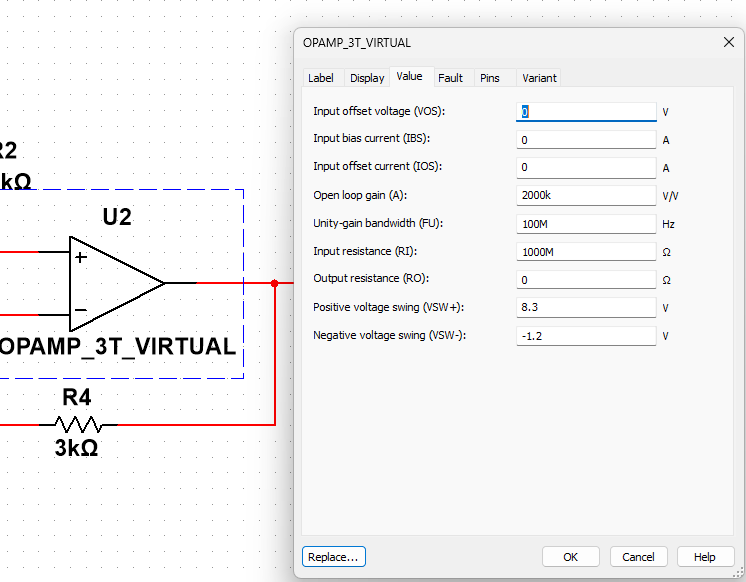
\includegraphics[width=.4\linewidth]{./my-chapters/my-images/Question5/c/c_mophong.png}
	\caption{Setup giá trị cho OPAMP có $V_{OH} = 8.3\,\textsf{V}$ và $V_{OL} = -1.2\,\textsf{V}$, các thông số còn lại là lí tưởng.}
\end{figure}

\begin{figure}[H]
	\centering
	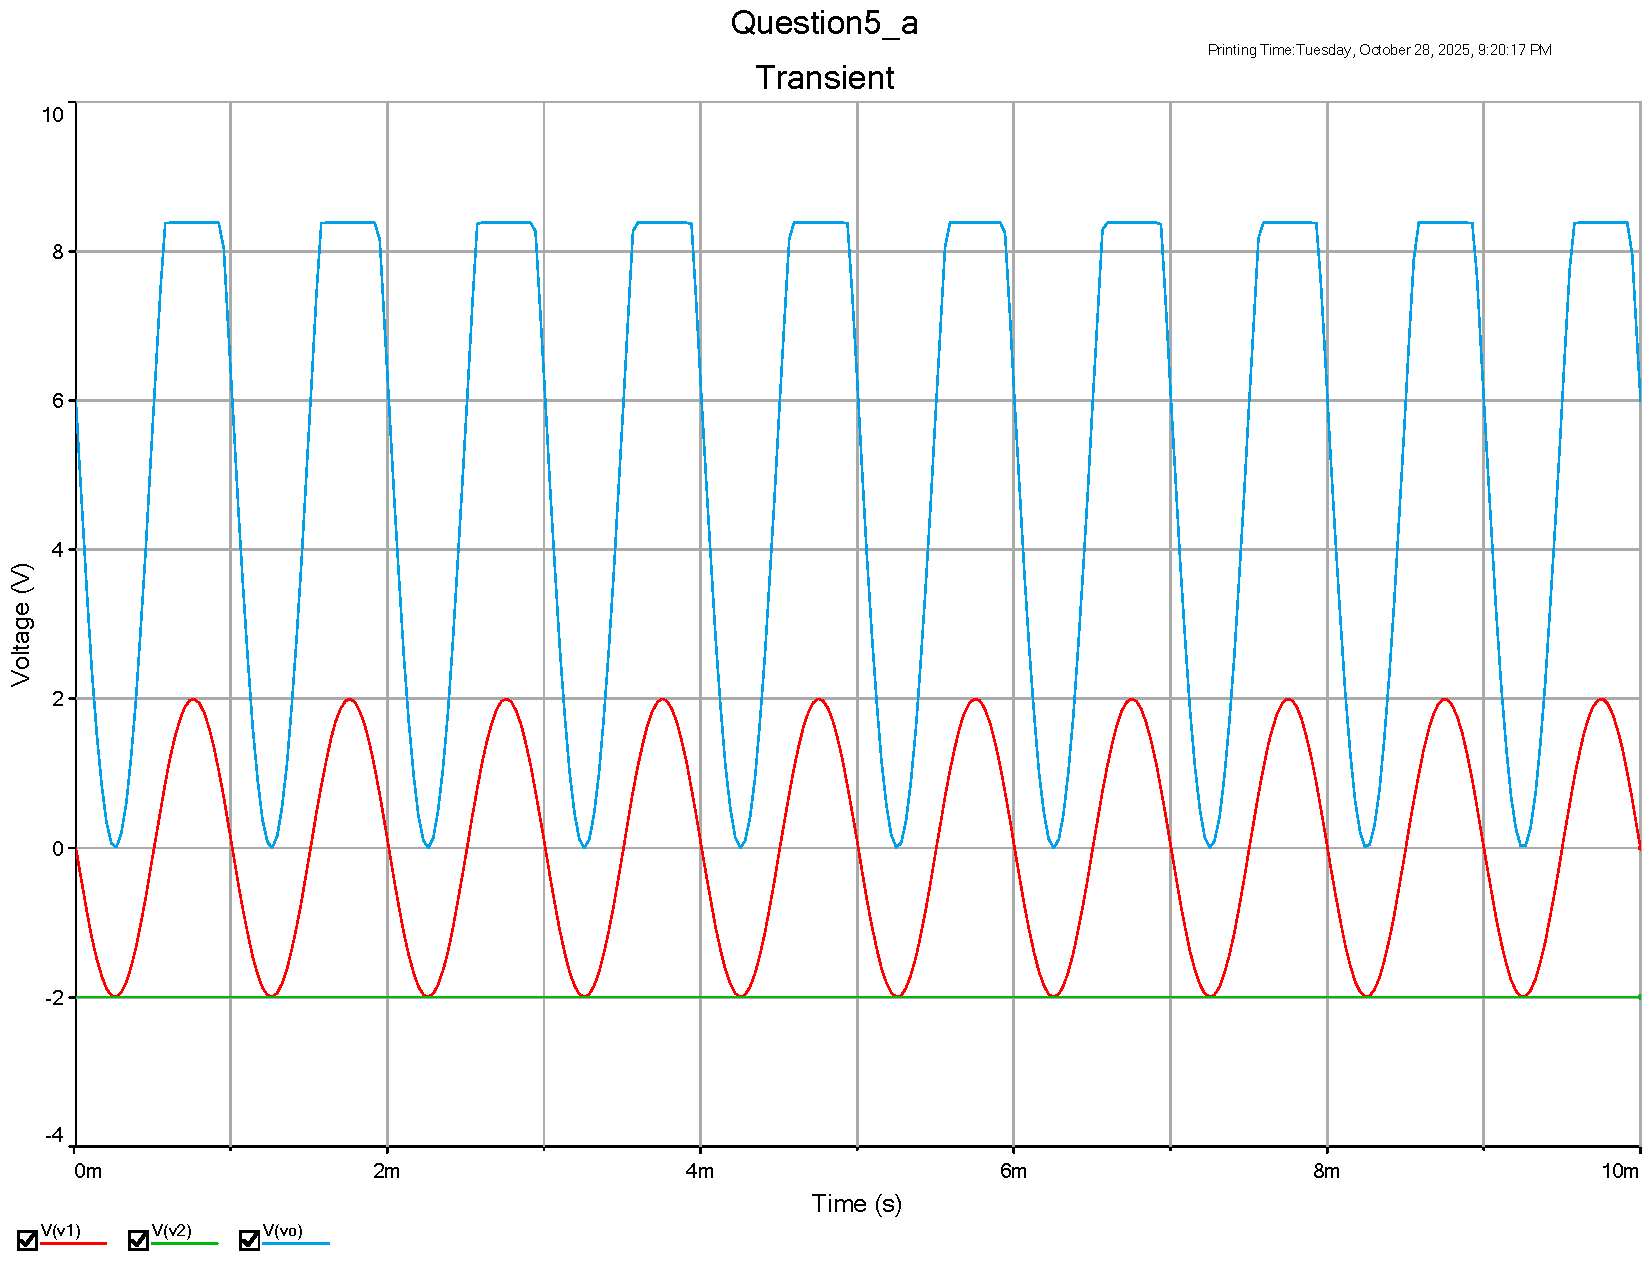
\includegraphics[width=.8\linewidth]{./my-chapters/my-diagrams/Question5/c_dangsongngora.pdf}
	\caption{Dạng sóng ngõ ra nếu OPAMP là lý tưởng.}
\end{figure}

Vì giá trị ngõ ra $V_{o}$ không có giá trị âm nên khi $V_{OL}$ giảm còn $-1.2\,\textsf{V}$ thì ngõ ra không bị ảnh hưởng.